\section{Introduction}

Some of the important questions in cellular biology have to do with how the sizes of different parts of the cell, the organelles, are regulated.
Here we concentrate on modeling the growth of the Eukaryotic flagellum, an organelle that protrudes from the cell and is usually used for propulsion.
The choice of studying a flagellum has the advantage of restricting the problem to growth in only one dimension.
~\cite{bressloff}

\begin{figure}[!ht]
\centering
\parbox[t][2.3in][t]{4in}{
\hspace{1in}IFT Particles\\
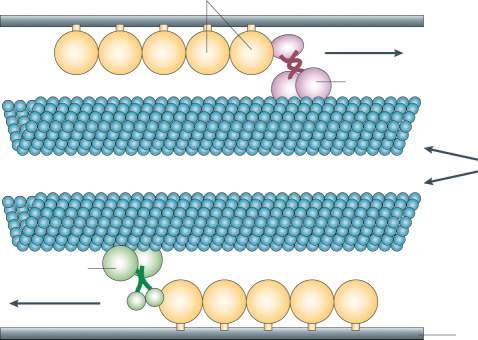
\includegraphics[width=3in]{IFT_diagram.png}
\raisebox{1.75in}[1pt][1pt]{\hspace{2.2in}Kinesin-II}\\
\raisebox{1.39in}[1pt][1pt]{\hspace{3.04in}Microtubules}\\
\raisebox{1.5in}[1pt][1pt]{($-$)\hspace{2.2in}($+$)}\\
\raisebox{1.05in}[1pt][1pt]{\hspace{-0.15in}Dynein-1b}\\
\raisebox{0.83in}[1pt][1pt]{\hspace{2.95in}Flagellar membrane}
}
\caption{The interflagellar transport machinery.~\cite{rosenbaum2}
During intraflagellar transport,
linear arrays of IFT particles (yellow) are anterograde,
towards the ($+$) ends of the flagellar microtubules (blue)
by kinesin-II (pink), and retrograde (towards the ($-$) ends)
by cytoplasmic dynein 1b (green).
The IFT particles carry precursors that are necessary for the assembly of
the flagellar axoneme.}
\end{figure}

Eukaryotic flagella grow using the mechanism of intraflagellar transport. This process describes the movement of particles (transporters) carrying building blocks (precursor proteins) along the microtubule and depositing them at the flagellum tip.
The transporters use different motors for anterograde (towards tip) movement and retrograde (towards cell body) movement.
~\cite{rosenbaum}

In order to express the length of the flagellum mathematically we define the relevant variables as follows:
$L$ represents the flagellar length, $a$ represents the effective size of a precursor protein transported by a transporter, $v_+$ represents a transporter's anterograde speed, $v_-$ represents a transporter's retrograde speed, and $M$ represents the number of transporters in the flagellum.
We also suppose that a flagellum degrades at a constant speed of $V$.
Using these parameters it is possible to arrive at an ordinary differential equation (ODE) for the flagellum length, at the microscopic level, however, a stochastic model may be more representative of the behavior of the motors and transporters.
Our goal is to represent flagellar growth as a stochastic process, and compare and contrast the stochastic model with the deterministic model.
We are also interested in analyzing the behavior that cannot be predicted by the deterministic model, such as the variation of the flagellum length.
The deterministic ODE for the flagellum length is:

\begin{equation*}
\frac{dL}{dt} = \frac{a \bar{v} M}{2L} - V
\end{equation*} 

Where $\bar{v}$ is the harmonic mean of $v_+$ and $v_-$.
The assembly rate, which is the positive right-hand-side term, is arrived at by noting that a transporter adds a segment of length $a$ to the flagellum every time it completes one round trip, to the tip of the flagellum and back.
The time it takes to complete this trip is the time taken to reach the tip from the base, $L/v_+$, added to the time it takes to reach the base from the tip, $L/v_-$, adding up to $2L/\bar{v}$.
The disassembly rate is given by $V$ and is length-independent.

The values we use for the parameters above in our simulations are taken from the paper by Paul C. Bressloff, \emph{Stochastic model of intraflagellar transport }~\cite{bressloff}: $v_+$, $v_-$, and $V$ are taken to be $2.0 \mu$m$/$s, $3.5 \mu$m$/$s, $0.01 \mu$m$/$s respectively, $M$ is taken to be 10, and $a$ is taken to be $10$nm.
